\chapter{Atividades desenvolvidas}

Este capítulo apresenta as atividades realizadas para a construção de um classificador binário capaz de identificar padrões de sintomas de doenças e categorizá-los  em enfermidades do tipo Dengue ou Chikungunya. Uma aplicação web também foi desenvolvida com o intuito de utilizar o modelo de classificação para que fosse possível gerar novas predições por meio de um \textit{browser} e exibir o resultado em páginas HTML (\textit{HyperText Markup Language}).

\section{Informações sobre as doenças}

\citeonline{laoprasopwattana2012differential} e \citeonline{lee2012simple} alegam que  a distinção entre casos de Dengue e Chikungunya é difícil de ser feita de forma eficaz apenas por observação porque os sintomas e sinais são bastante similares, sendo assim, é necessário realizar exames clínicos para obter um diagnóstico satisfatório. Nesse sentido, o uso de uma sistema computacional de apoio à decisão pode ser útil, por exemplo, para realizar a triagem inicial de pacientes em um hospital de maneira mais rápida e efetiva.

Existem pelo menos dois tipos de exames que podem ser utilizados para detecção de Dengue. São eles: o RT-PCR (\textit{Reverse transcription polymerase chain reaction}) e NS1 ELISA \cite{verma2016evaluation}. Os dois exames possuem características distintas para a detecção do vírus da dengue, no Brasil o exame que utiliza o NS1 Elisa é realizado por meio do Sistema Único de Saúde (SUS) desde agosto de 2017\footnote{\url{http://pesquisa.in.gov.br/imprensa/jsp/visualiza/index.jsp?jornal=1&pagina=56&data=10/08/2017}}. \citeonline{mata2014} realizaram um estudo comparativo entre os exames de teste rápido do tipo NS1 ELISA a fim de detectar a precisão de cada um. O estudo concluiu que a precisão dos exames pode variar entre 55,8 a 83,4\%, o que pode culminar na alta equivocada de pacientes. O valor destes exames pode variar de R\$ 13,00 a R\$ 28,00.

\citeonline{Cecilia2015} demonstram em seu estudo um exame do tipo RT-PCR capaz de detectar dengue e chikungunya com taxas de assertividade de 95\% a 100\% respectivamente. Diferentemente dos exames utilizados pelo SUS, o RT-PCR é mais caro que um semelhante como o NS1 ELISA e também necessita de melhores aparatos laboratoriais \cite{verma2016evaluation}.

\citeonline{Huang2013} demonstram a perda de eficácia para os exames do tipo NS1 ELISA à medida que os dias de infecção passam e isto é um agravante no caso dos usuários do SUS já que o manual de diagnóstico e manejo para a dengue\footnote{\url{http://bvsms.saude.gov.br/bvs/publicacoes/dengue_diagnostico_manejo_adulto_crianca_3ed.pdf}} recomenda a realização do exame clínico a partir do sexto dia de início dos sintomas.

Diante das dificuldades e limitações existentes na triagem de pacientes e, considerando que nem sempre exames podem ser realizados rápida e eficazmente, busca-se, por meio de sinais e sintomas identificados, realizar a classificação proposta neste trabalho. A metodologia aplicada é explicada a seguir.

\section{Metodologia}
Sabendo que os sinais e sintomas apresentados pelas duas doenças são semelhantes e que a distinção entre as duas por meio de uma observação empírica é dificultada por tais características, foi proposta uma hipótese de investigação. A hipótese definida foi:

\textit{É possível realizar a classificação entre duas doenças com sinais e sintomas similares, descritos apenas de forma binária como "sim ou não", de modo que a probabilidade de acerto seja igual ou superior a 80\%?}

A porcentagem de 80\% para a precisão de acerto foi definida levando em consideração os exames clínicos existentes, onde os exames mais acessíveis possuem média semelhante para a detecção das duas doenças.

Para a execução deste trabalho as etapas a seguir foram realizadas:

\begin{enumerate}[label=\roman*]
 \item Levantamento do estado da arte;
 \item Obtenção de dados sobre Dengue e Chikungunya;
 \item Compreensão dos dados sobre Dengue e Chikungunya;
 \item Seleção, pré-processamento, integração e persistência dos dados;
 \item Estudo de algoritmos de classificação;
 \item Aplicação de algoritmos de classificação;
 \item Avaliação dos resultados;
 \item Construção de uma aplicação que permita a interação com o classificador
\end{enumerate}


\section{Dados sobre as arboviroses}

A concepção do modelo de classificação - objeto deste trabalho - utilizou um conjunto de dados de pacientes da rede pública de atendimento do estado da Paraíba, concedidos pela Secretaria da Saúde do Estado da Paraíba (SES-PB). Os dados fornecem informações sobre os pacientes com suspeita ou com a confirmação de Dengue e Chikungunya no ano de 2016.

Os dados, disponibilizados em formato de arquivo CSV, compreendem entre 156 e 159 atributos de informação (colunas no arquivo), para dengue e chikungunya respectivamente. Os atributos variam desde a localidade de moradia do paciente até o resultado de exames realizados. A Figura \ref{fig:csvses} exibe um fragmento do \textit{dataset}, onde é possível observar que existem instâncias com dados não informados como também é possível observar o tipo de informação que as colunas possuem (o valor 1 representa SIM e o valor 2 representa NÃO).

\begin{figure}[htb]
  \caption{\label{fig:csvses}Fragmento de informação sobre doenças}
  \begin{center}
    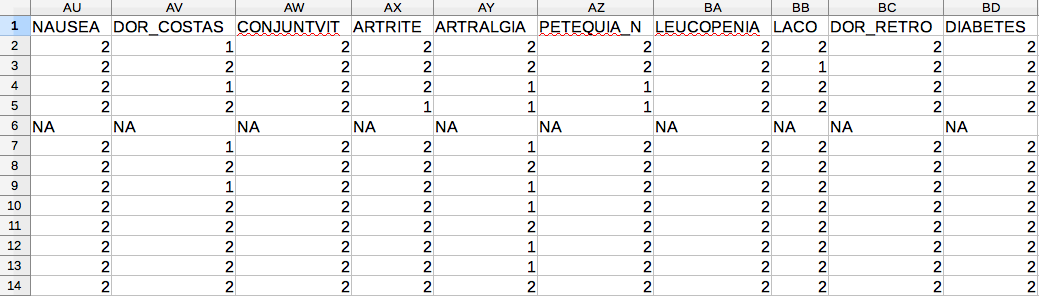
\includegraphics[width=\textwidth]{imagens/fragmentodosdados.png}
    \legend{Fonte: SES-PB}
  \end{center}
\end{figure}

Inicialmente, foi necessário analisar o conjunto de metadados para entender o contexto das informações inerentes ao domínio das arboviroses (Dengue e Chikungunya), visto que, por algumas vezes, os nomes dos atributos não eram claros o suficiente para expressar o seu significado. Para contornar este problema, utilizamos os metadados fornecidos pelo portal de dados abertos da cidade do Recife\footnote{\url{http://dados.recife.pe.gov.br/dataset/rede-de-saude-municipal}}, que também permite acesso a um conjunto dados sobre as doenças investigadas na cidade do Recife. A Figura \ref{fig:metadados} exibe um fragmento dos metadados fornecidos pelo portal, onde é possível observar que as informações também não são conclusivas, porém é de grande ajuda a detecção do grupo de informação ao qual um atributo pertence.

\begin{figure}[htb]
  \caption{\label{fig:metadados}Fragmento dos metadados sobre sinais e sintomas das doenças}
  \begin{center}
    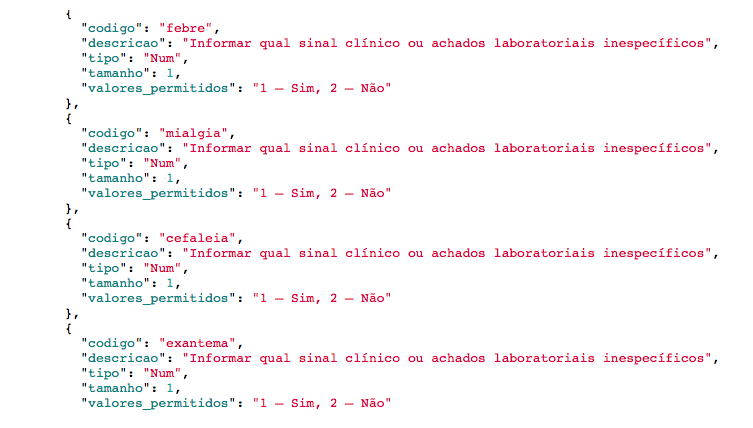
\includegraphics[width=\textwidth]{imagens/fragmentodosmetadados.png}
    \legend{Fonte: Portal de dados abertos do Recife}
  \end{center}
\end{figure}
\newpage

\section{Preparação do conjunto de dados}

As etapas de seleção, pré-processamento e transformação do KDD foram aplicadas aos dados fornecidos pela SES-PB. Na fase de seleção, foram removidos do \textit{dataset} os dados sobre outras doenças fora do contexto deste trabalho como também os atributos que em nada contribuíram durante a fase de mineração, como, por exemplo, a cidade do paciente.

Durante a etapa de pré-processamento, foi necessário efetuar a normalização de datas para um formato único. Também foram removidas instâncias que não possuíam as informações completas sobre o quadro de sinais e sintomas das doenças. Nesta etapa também foram retiradas do \textit{dataset} as instâncias que estavam marcadas como casos descartados ou inconclusivos. Inicialmente o \textit{dataset} contava com 58.657 instâncias sobre os pacientes e, após a etapa de pré-processamento, 17.205 instâncias restaram. De uma média de 157 atributos apenas 21 foram mantidos (febre, mialgia, cefaleia, exantema, vômito, náusea, dor nas costas, conjuntivite, artrite, artralgia, auto imune, petéquia, leucopenia, prova do laço, dor retro-orbitária, diabetes, hematolog, hepatopatia, doenças renais, hipertensão, ácido péptico). Os 21 atributos mantidos são os sinais e sintomas dos pacientes para cada doença e foram mantidos porque apenas estes fazem parte do contexto do problema (classificação por meio de sinais e sintomas).

Na etapa  de transformação, os dados foram mantidos em dois formatos distintos para posterior utilização: CSV e ARFF. Para realizar a transformação do arquivo CSV em um arquivo ARFF foi construído um script na linguagem Python capaz de produzir um arquivo ARFF a partir dos dados e metadados de um arquivo CSV.

O Quadro \ref{quadro:arff} exibe um fragmento do arquivo de tipo ARFF criado a partir das informações do arquivo CSV. É possível observar que a estrutura do arquivo é bem definida com espaços para nomear o \textit{dataset}, registrar os atributos, marcar os tipos de dados para cada atributo e registrar as informações propriamente ditas sobre o conjunto de dados, ou seja, seus valores.

\begin{quadro}
\caption{\label{quadro:arff}Fragmento do arquivo ARFF}
\begingroup
    \fontsize{10pt}{9pt}\selectfont
    \begin{verbatim}  
@RELATION dengue-chikungunya

@ATTRIBUTE FEBRE Numeric
@ATTRIBUTE MIALGIA Numeric
@ATTRIBUTE CEFALEIA Numeric
@ATTRIBUTE EXANTEMA Numeric
@ATTRIBUTE VOMITO Numeric
@ATTRIBUTE NAUSEA Numeric
@ATTRIBUTE DOR_COSTAS Numeric
@ATTRIBUTE CONJUNTVIT Numeric
@ATTRIBUTE ARTRITE Numeric
@ATTRIBUTE ARTRALGIA Numeric
@ATTRIBUTE PETEQUIA_N Numeric
@ATTRIBUTE LEUCOPENIA Numeric
@ATTRIBUTE LACO Numeric
@ATTRIBUTE DOR_RETRO Numeric
@ATTRIBUTE DIABETES Numeric
@ATTRIBUTE HEMATOLOG Numeric
@ATTRIBUTE HEPATOPAT Numeric
@ATTRIBUTE RENAL Numeric
@ATTRIBUTE HIPERTENSA Numeric
@ATTRIBUTE ACIDO_PEPT Numeric
@ATTRIBUTE AUTO_IMUNE Numeric
@ATTRIBUTE CLASS {chikungunya,dengue}

@DATA
0,1,0,1,0,0,1,0,0,1,0,0,0,0,0,0,0,0,0,0,0,chikungunya
1,1,1,1,1,1,0,0,0,1,0,0,0,1,0,0,0,0,0,0,0,dengue
1,1,1,1,0,0,1,0,0,1,0,0,0,0,0,0,0,0,0,0,0,dengue
    \end{verbatim}  
\endgroup
\legend{Fonte: O autor}
\end{quadro}
\newpage

\section{O processo de classificação e algoritmos utilizados}

A tarefa de classificação foi escolhida para ser analisada no processo de mineração de dados porque nós já havíamos iniciado outro processo de classificação com dados similares, dessa forma existia uma certa familiaridade com tal tarefa. Com os dados previamente consolidados, o processo de criação do classificador pôde ser iniciado. Nesta etapa a hipótese foi investigada exaustivamente, também foram analisados os parâmetros de sensitividade e especificidade resultantes de cada classificação. Os três algoritmos escolhidos para a realização da classificação foram Naive bayes, \textit{Support Vector Machine} (SVM) e \textit{Classification and Regression Trees} (CART). Estes são algoritmos bastante utilizados em áreas como agricultura, medicina e geologia \cite{dong2014nonlinear}.

Assim que a etapa de transformação dos dados foi finalizada, o processo de classificação pôde ser iniciado. A linguagem R foi utilizada para treinar e testar os modelos de classificação. Para treinamento dos algoritmos foram utilizadas as 17.205 instâncias resultantes da fase de pré-processamento dos dados (100\% dos dados), e foi utilizado o método \textit{k-fold Cross-Validation} com o número de \textit{fold} definido em 10 ($k = 10$). As próximas seções (3.5.1, 3.5.2, 3.5.3, 3.5.4) demonstram o processo de classificação para cada um dos algoritmos escolhidos para este experimento, bem como seu respectivo desempenho, e a Seção 3.5.5 condensa as informações apresentadas com uma análise final para os resultados.

\subsection{Naive Bayes}
O classificador Naive Bayes é um dos mais utilizados no aprendizagem de máquina por causa da sua simplicidade, velocidade para treinamento e capacidade em aprender sobre problemas complexos \cite{dong2014nonlinear,zhang2004optimality,chakrabarti2002mining}. Trata-se de um algoritmo fundamentado no teorema de Bayes para classificação probabilística. O teorema determina a probabilidade de acontecimento para uma classe de acordo com as observações de dados anteriores \cite{Aggarwal2015}. Desta forma, é possível atualizar a probabilidade de um evento após investigar as evidências sobre o mesmo. O teorema recebe este nome não só por causa do seu descobridor (Thomas Bayes) mas também por ser considerado ingênuo (\textit{naive}) pela sua suposição de que todas as variáveis de um problema são independentes condicionalmente, sendo assim o acontecimento de um evento não deve influenciar na ocorrência de outros conjuntos de eventos para outras variáveis.

O primeiro teste de classificação foi realizado utilizando o algoritmo Naive Bayes, onde os parâmetros para treinamento foram os 21 sinais e sintomas (febre, mialgia, cefaleia, exantema, vômito, náusea, dor nas costas, conjuntivite, artrite, artralgia, auto imune, petéquia, leucopenia, prova do laço, dor retro-orbitária, diabetes, hematolog, hepatopatia, doenças renais, hipertensão, ácido péptico) para as duas doenças. A matriz de confusão pode ser vista no Quadro \ref{quadro:naivematriz1}.

\begin{quadro}
\caption{\label{quadro:naivematriz1}Matriz de confusão do algoritmo Naive Bayes}
\begingroup
    \fontsize{10pt}{9pt}\selectfont
    \begin{Verbatim}[commandchars=\\\{\}]
      Confusion Matrix and Statistics
                    Reference
       Prediction      dengue  chikungunya
       dengue            \textbf{9244}       5389
       chikungunya       791        \textbf{1781}
                                         
               Accuracy : 0.6408         
                 95% CI : (0.6336, 0.648)
     \textbf{Sensitivity/Recall} : 0.9212         
            \textbf{Specificity} : 0.2484         
      \textbf{Balanced Accuracy} : 0.5848
              F-measure : 0.7494        
         
       'Positive' Class : dengue 
       'Negative' Class : chikungunya
  
    \end{Verbatim}  
\endgroup
\legend{Fonte: O autor}
\end{quadro}
\newpage

Por meio do Quadro \ref{quadro:naivematriz1} é possível observar que a precisão balanceada foi de 58,48\%, ou seja, o algoritmo foi capaz de acertar 58,48\% das vezes para o nosso conjunto de dados. É importante ressaltar que apenas essa medida não é suficiente para informar se um algoritmo é bom ou ruim para o conjunto dos dados, é preciso observar também as medidas como \textit{sensitivity} e \textit{specificity}.

É possível observar no Quadro \ref{quadro:naivematriz1} que o algoritmo Naive Bayes foi muito enfático para determinar quais instâncias pertenciam ao conjunto da Dengue. Conforme resultado da medida de sensitividade (\textit{sensitivity} ou \textit{recall}), em 92,12\% das instâncias o algoritmo classificou corretamente os casos de dengue. Entretanto a medida de especificidade (\textit{specificity}) demonstra que o algoritmo acertou apenas 24,84\% dos casos para a Chikungunya. De uma maneira geral o algoritmo não obteve a performance necessária para validar a hipótese do trabalho e demonstrou uma certa tendência para classificar as instâncias como Dengue, o que, por sua vez, pode ser um aspecto perigoso quando tratamos de identificar doenças.

\subsection{\textit{Classification and Regression Trees}}

O CART representa uma árvore de decisão binária e recursiva de particionamento capaz de processar valores numéricos e nominais como atributos e classes \cite{steinberg2009cart}. O processo de particionamento começa com um nó central que posteriormente é dividido em mais dois nós filhos, e os particionamentos seguem até que não haja mais a possibilidade para divisões, o CART permite a criação de várias árvores de decisão a fim de eleger uma árvore que possua o melhor balanço entre o \textit{overfitting} e o \textit{underfitting}. Informações mais detalhadas sobre o CART podem ser vistos em \citeonline{breiman2017classification}.

Assim como no processo de classificação com o Naive Bayes, foram utilizados os 21 atributos. O Quadro \ref{quadro:cart1} demonstra o resultado da classificação utilizando o CART.


\begin{quadro}
\caption{\label{quadro:cart1}Matriz de confusão do algoritmo CART}
\begingroup
    \fontsize{10pt}{9pt}\selectfont
    \begin{Verbatim}[commandchars=\\\{\}]
      Confusion Matrix and Statistics
                    Reference
       Prediction      dengue  chikungunya
       dengue            \textbf{7981}       2835
       chikungunya       2054        \textbf{4335}
                                         
               Accuracy : 0.7158         
                 95% CI : (0.709, 0.7226)
     \textbf{Sensitivity/Recall} : 0.7953         
            \textbf{Specificity} : 0.6046         
      \textbf{Balanced Accuracy} : 0.7000
              F-measure : 0.7655        
         
       'Positive' Class : dengue 
       'Negative' Class : chikungunya
  
    \end{Verbatim}  
\endgroup
\legend{Fonte: O autor}
\end{quadro}

É possível observar que a precisão balanceada é de 70.00\%, ou seja, 11.52\% mais alta que o Naive Bayes, entretanto também precisamos observar as outras estatísticas derivadas do processo. Para a classificação de instâncias com o rótulo real de Dengue (sensitividade), o algoritmo obteve uma precisão de 79.53\%, representando uma redução de 12.59\% em comparação com o Naive Bayes. A classificação de instâncias com o rótulo de Chikungunya (especificidade) obteve uma performance de 60.46\%, o que representa 35.62\% acima do Naive Bayes.

De uma maneira geral, o CART obteve uma performance consideravelmente superior ao Naive Bayes. Com a precisão média em 70.00\%, o CART não atingiu a performance mínima esperada pela hipótese do trabalho.

\subsection{\textit{Support Vector Machine}}

O \textit{Support Vector Machine} (SVM) é um algoritmo de aprendizagem de máquina, do tipo supervisionado, que cria vetores em um espaço de hiperplanos por meio dos atributos dos dados de treinamento a fim de criar uma separação entre instâncias de classes diferentes \cite{rebentrost2014quantum}. No caso da classificação, a separação é feita em exemplos positivos e negativos. A idéia básica é encontrar o hiperplano de separação ideal entre os exemplos positivos e negativos.

A Figura \ref{fig:svm} demonstra um exemplo para a classificação de instâncias onde o hiperplano é do tipo linear, é possível observar a margem de separação entre os grupos de cada classes, como também é possível observar os vetores de suporte que cruzam as instâncias no plano (X, Y).

\begin{figure}[htb]
  \caption{\label{fig:svm}Hiperplanos de separação e Vetores de suporte }
  \begin{center}
    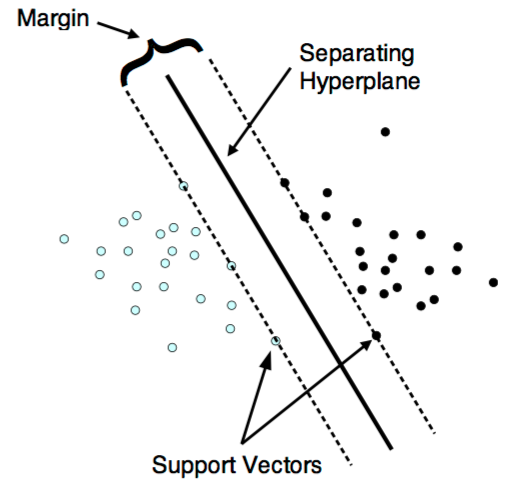
\includegraphics[scale=0.4]{imagens/svm.png}
    \legend{Fonte: \citeonline{Meyer2017}}
  \end{center}
\end{figure}
\newpage

O hiperplaneiro ideal pode ser obtido maximizando a margem entre dois hiperplanos paralelos \cite{qi2013robust}. Esta é uma técnica  poderosa e muito utilizada para gerar modelos de classificação \cite{Meyer2017}. Mais informações sobre o embasamento teórico e funcionamento do algoritmo podem ser encontradas no trabalho de \citeonline{cortes1995support}.

Assim como nos exemplos com o Naive Bayes e CART, foi gerado um modelo de classificação utilizando o SVM. A O Quadro \ref{quadro:svm1} exibe a matriz de confusão e as estatísticas de classificação. É possível observar que a precisão média é ligeiramente superior (2.35\%) à média apresentada pelo CART, a sensitividade é 6.28\% inferior e a precisão em classificar a Chikungunya é 10.99\% maior.

\begin{quadro}
\caption{\label{quadro:svm1}Matriz de confusão do algoritmo SVM}
\begingroup
    \fontsize{10pt}{9pt}\selectfont
    \begin{Verbatim}[commandchars=\\\{\}]
      Confusion Matrix and Statistics
                    Reference
       Prediction      dengue  chikungunya
       dengue            \textbf{7351}       2047
       chikungunya       2684        \textbf{5123}
                                         
               Accuracy : 0.725         
                 95% CI : (0.7183, 0.7317) 
     \textbf{Sensitivity/Recall} : 0.7325         
            \textbf{Specificity} : 0.7145         
      \textbf{Balanced Accuracy} : 0.7235
              F-measure : 0.7565        
         
       'Positive' Class : dengue 
       'Negative' Class : chikungunya
  
    \end{Verbatim}  
\endgroup
\legend{Fonte: O autor}
\end{quadro}


\subsection{Experimentação aplicando a técnica de Seleção de Atributos}

Como foi discutido anteriormente, os sinais e sintomas apresentados pelos pacientes são muito parecidos. Dois pacientes com os mesmos sintomas podem ter doenças diferentes (entre Dengue e Chikungunya). Este fenômeno é conhecido na mineração de dados como overlapping ou sobreposição de classes \cite{xiong2010classification}.

A sobreposição de classes dificulta o trabalho do algoritmo de classificação, visto que fica mais difícil identificar corretamente a qual classe uma instância pertence. Como \citeonline{martin2009suitability} sugerem, existem técnicas específicas para tratar este problema, algumas das técnicas sugeridas são a seleção de atributos específicos por correlação\footnote{É uma técnica verifica quais atributos possuem uma correlação alta ou moderada em relação a classe e uma baixa correlação entre os outros atributos \citeonline{hall1999correlation}.} e ganho de informação\footnote{O ganho de informação técnica que visa selecionar os atributos de um \textit{dataset} que mais contribuem para o aumento do desempenho de um algoritmo de predição.}.


A fim de observar mais de perto o domínio dos dados nós realizamos experimentos com a seleção de atributos utilizando a ferramenta Weka. Foi aplicada a técnica de seleção de atributos por meio da medida de ganho de informação. O Weka criou um ranking com os atributos mais relevantes para a predição da classe das doenças e, ao seu término,  7 dos 21 atributos foram selecionados, onde, em teoria, os sintomas descartados não devem impactar negativamente no desempenho dos classificadores. Os sintomas selecionados podem ser vistos na Tabela \ref{tab:7colunas}. 

Logo após a seleção dos atributos mais relevantes, o processo de classificação foi reiniciado com os mesmos algoritmos dos testes iniciais. Nos testes com o algoritmo Naive Bayes foi detectada uma melhora de performance de 4.54\%, o algoritmo CART obteve uma performance de 68.78\% (uma perda de 1.22\%), e o algoritmo SVM obteve uma performance de 68.39\%, uma perda de 3.96\% em sua precisão média. As matrizes de confusão podem ser consultadas no \textbf{Apêndice A}.


\begin{table}[h]
\begin{center}
\caption{\label{tab:7colunas}Sinais e sintomas selecionados para classificação}

\begin{tabular}{c|c|c|c}
\hline 
Artralgia & Dor nas costas & Conjuntivite & Artrite \\ 
\hline 
Náuseas & Exantema & Hipertensão & • \\ 
\hline 
\end{tabular} 

\legend{Fonte: O autor}

\end{center}
\end{table}
\newpage

\subsection{Análise geral da classificação}

Com o fim do processo de classificação foi possível quantificar qual algoritmo obteve uma melhor precisão balanceada para o nosso conjunto de dados. O algoritmo de \textit{Support Vector Machine} obteve a melhor performance nas primeiras rodadas de teste, e o algoritmo CART obteve a melhor performance após a seleção de atributos. A Figura \ref{fig:precisoesbalanceadas} exibe as precisões médias de classificação para as duas iterações.

\begin{figure}[htb]
  \caption{\label{fig:precisoesbalanceadas}Precisão balanceada para classificação}
  \begin{center}
    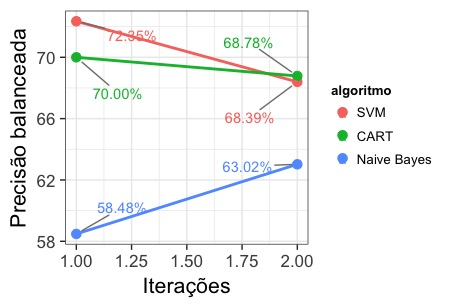
\includegraphics[scale=0.7]{imagens/atributos_selecao_desempenho_linhas.jpeg}
    \legend{Fonte: O Autor}
  \end{center}
\end{figure}

De uma maneira geral, os três algoritmos não obtiveram a medição  mínima de desempenho para validar a hipótese. Entendemos que a natureza do problema de classificação abordado neste trabalho não demanda uma solução trivial, e é necessário especializar o processo de classificação direcionado às particularidades do problema.

Fatores como o desbalanceamento do \textit{dataset} e \textit{overlapping} de classes impactaram diretamente os resultados apresentados, outros fatores como atributos binários não ajudam para a detecção da borda de decisão. Para clarificar este entendimento podemos ter como exemplo a possibilidade de que o sinal de febre seja mais acentuado em uma doença que em outra, sendo assim, esta característica poderia vir a ajudar numa melhor classificação. A obtenção de atributos adicionais e relevantes para identificação  das  duas doenças poderá ajudar na melhoria do desempenho  dos classificadores. Ainda assim, é necessário levar em consideração que mesmo com mais dados há o risco da borda que separa estas duas doenças não ser suficientemente clara para as técnicas selecionadas para a classificação.

\section{Aplicação Web (ArboML)}

Após a criação do classificador foi iniciado o processo de especificação e implementação de uma aplicação que permita a interação com o mesmo e que tornasse fácil o acesso e visualização do resultado. Foi escolhido implementar uma interface que pudesse ser acessada por meio dos \textit{browsers} e da internet e que não fosse preciso instalar nada no dispositivo de acesso.

A Figura \ref{fig:arboml} exibe a implementação da interface de classificação sendo acessada por um navegador como também sinais e sintomas selecionados e o resultado da classificação ao lado. O funcionamento da interface é bem simples: o usuário pode selecionar quais sinais e sintomas são apresentados, e o resultado da predição é atualizado em tempo real. Toda a comunicação entre o classificador e a interface ArboML é feito via protocolo HTTP com chamadas assíncronas a um servidor que mantém o classificador online.

\begin{figure}[htb]
  \caption{\label{fig:arboml}ArboML}
  \begin{center}
    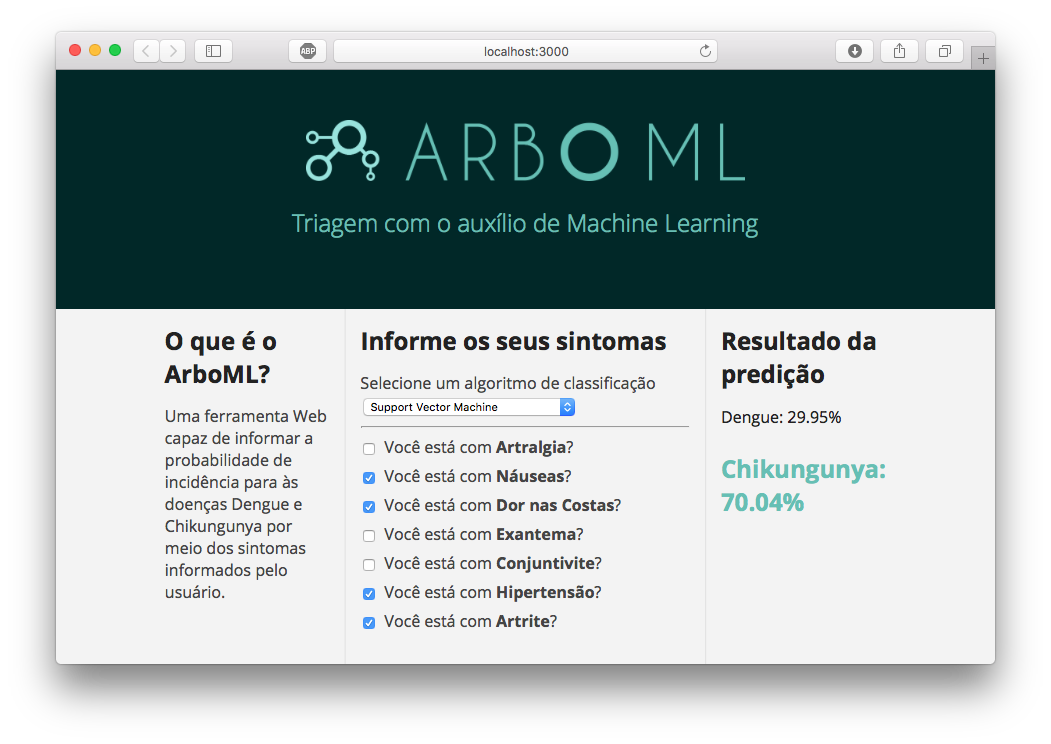
\includegraphics[scale=0.46]{imagens/arboML.png}
    \legend{Fonte: O Autor}
  \end{center}
\end{figure}
\newpage

A ArboML foi implementada utilizando tecnologias como HTML, \textit{Cascading Style Sheets} (CSS) e JavaScript onde o principal foco é o JavaScript que é responsável em fazer as chamadas ao servidor do classificador. A princípio, a ArboML tem o intuito de apresentar  apresentar o resultado da classificação de forma simples, clara e objetiva ao usuário final. A precisão da classificação da doença é determinada pela avaliação de desempenho dos classificadores. Não faz parte do escopo deste trabalho uma avaliação qualitativa da usabilidade da ArboML, tendo em vista que foram detectadas necessidades de trabalhos futuros para aprimoramento da metodologia utilizada neste trabalho, cujo foco se concentra nas atividades de mineração em si. A aplicação e seus aspectos de usabilidade serão futuramente estendidas.

A Figura \ref{fig:api} demonstra a arquitetura de acesso aos classificadores por meio de uma API que utiliza o protocolo HTTP para expor a interface de acesso aos classificadores produzidos neste trabalho.

\begin{figure}[htb]
  \caption{\label{fig:api}Arquitetura de interação com o classificador}
  \begin{center}
    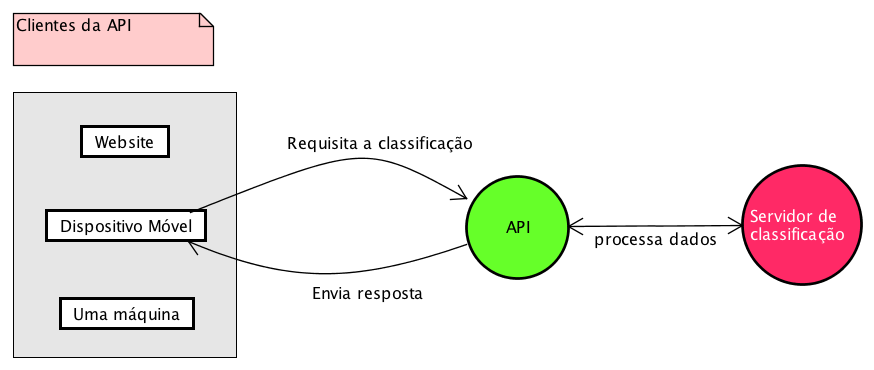
\includegraphics[scale=0.7]{imagens/api-diagram.png}
    \legend{Fonte: O Autor}
  \end{center}
\end{figure}
\newpage
